%%%%%%%%%%%%%%%%%%% author.tex %%%%%%%%%%%%%%%%%%%%%%%%%%%%%%%%%%%
%
% sample root file for your "contribution" to a contributed volume
%
% Use this file as a template for your own input.
%
%%%%%%%%%%%%%%%% Springer %%%%%%%%%%%%%%%%%%%%%%%%%%%%%%%%%%


% RECOMMENDED %%%%%%%%%%%%%%%%%%%%%%%%%%%%%%%%%%%%%%%%%%%%%%%%%%%
\documentclass[graybox]{svmult}

% choose options for [] as required from the list
% in the Reference Guide

\usepackage{mathptmx}       % selects Times Roman as basic font
\usepackage{helvet}         % selects Helvetica as sans-serif font
\usepackage{courier}        % selects Courier as typewriter font
\usepackage{type1cm}        % activate if the above 3 fonts are
                            % not available on your system
%
\usepackage{makeidx}         % allows index generation
\usepackage{graphicx}        % standard LaTeX graphics tool
                             % when including figure files
\usepackage{multicol}        % used for the two-column index
\usepackage[bottom]{footmisc}% places footnotes at page bottom
% see the list of further useful packages
% in the Reference Guide

\makeindex             % used for the subject index
                       % please use the style svind.ist with
                       % your makeindex program

%%%%%%%%%%%%%%%%%%%%%%%%%%%%%%%%%%%%%%%%%%%%%%%%%%%%%%%%%%%%%%%%%%%%%%%%%%%%%%%%%%%%%%%%%

\begin{document}

\title*{Predication Instances spot price in EC2}
\author{test test}
\institute{Name of First Author \at Name, Address of Institute, \email{name@email.address}
\and Name of Second Author \at Name, Address of Institute \email{name@email.address}}
%
% Use the package "url.sty" to avoid
% problems with special characters
% used in your e-mail or web address
%
\maketitle

\abstract{We analyze G2 spot instance price}

\section{Introduction}\label{sec:1}
Cloud computing provides various types of compute resources to serve diverse application scenarios. The cloud computing frees the burden of system administration overheads without incurring prohibitive initial hardware purchase cost. From the service provider's perspective, fully utilizing the already established hardware resources and services is crucial to maximize monetary gain. As the users' resource demand can vary from time to time, some cloud computing providers offer services at chaper price than the regular price to maximize hardware/service utilization. For instance, Amazon Web Services (AWS), a leading cloud computing vendor, provides its surplus of EC2 computing resources at a cheaper price in the form of \emph{spot instance}. A user who wants to use spot instance bids for a price that one is willing to pay, and if the bid price is higher than the spot price that is decided by the service provider, one can get the resource allocated and pays for the spot price in the hourly basis. Other than AWS, Google Cloud Engine provides such opportunistic resources in the form of \emph{preemptive instances}, and Microsoft Azure provides its excess compute capacity as \emph{low-priority VM}.

Though users can utilize the opportunistic resources at a cheaper price, sudden service termination can happen at anytime as the demand for the computing resource changes. To mitigate the chance of sudden service interruption, few works were conducted to better predict and model the price change of EC2 spot instance in literature. Ben-Yehuda et al.~\cite{spot-instance-pricing-analysis} and Zhao et al.~\cite{spot-price-han-arima} tried to predict the future spot instance price using various predictive analysis algorithms, but they all concluded that the spot price is rather random and hard to make meaningful prediction for future price changes. Since then, most of studies that are related to the utilization of spot instance focus on the handling sudden service interruption~\cite{tr-spark,spot-mpi-checkpoint,flint,deep-spot-cloud} or spot instance bid strategy~\cite{not-bid-cloud,how-to-bid-cloud}. 

In this paper, we apply few time-series analysis algorithms to predict future price change pattern of AWS EC2 spot instances. By carefully desiging the period of train datasets, we could uncover that applying seasonal-arima (s-arima) can improve the accuracy of price change prediction error by XY\% comparing to the naive method that references most recent price to predict future price~\cite{deep-spot-cloud}. In addition to the contribution of improved price prediction accuracy, we could also discover that the configuration values to get the best prediction accuracy differs significantly across different availability zones (AZs) and instance types. Based on the extensive experiments and promising results, we bring up an opportunity of improving spot instance prediction accuracy that can result in significant cost gain for cloud computing users with increased system stability.


\section{Time-Series Analysis for GPU Spot Instances}
List basic methods that are widely used in other wors
focus to analyze the predication of spot instances price for 7 regions by use different time series models such as ARIMA, SARIMA VAR, DLM, prophet, average and naïve model
our work covered  7 regions of spot instances datasets, ap-northeast-1, ap-southeast-1, ap-regions, and 5 types and different period of datasets G2(03-02 to 2016-10-31),I2(2016-05-03 to 2017-02-04),M4,c3,R3(2016-03-02 to 2017-02-04)


naive

mean

seasonal mean

ARIMA with different parameters 
stander for Autoregressive Integrated Moving Average, which is the most popular statistical model and widely used to forecasting a time series, the model is a combination of  autoregressive Eq.~\ref{Eq-AR} and moving-average model Eq.~\ref{Eq-MA}, with three parameters  (p,d,q) where p is the number of autoregressive terms, which is depends on past values, d is the degree of differencing and q is the number of lagged forecast errors in the prediction equation, depends only on the random error terms 
\begin{equation}
 y_t = w_0 +\beta_1 y_{t-1}+ \beta_2 y_{t-2}+.....\beta_n y_{t-n}+\epsilon_t
\label{Eq-AR}
\end{equation}


\begin{equation}
 y_t = w_0 +\epsilon_t + \delta_1 \epsilon_{t-1}+  \delta_2 \epsilon_{t-2}+...+ \delta_n \epsilon_{t-n}
\label{Eq-MA}
\end{equation}

Thus, ARIMA if d=n will be 
\begin{equation}
 y_t = w_0 +\beta_1 y_{t-1}+ \beta_2 y_{t-2}+.....\beta_n y_{t-n} +  \delta_1 \epsilon_{t-1}+  \delta_2 \epsilon_{t-2}+...+ \delta_n \epsilon_{t-n}+
\label{Eq-ARIMA}
\end{equation}
Where the term \(\beta_i \) is, weight applied to prior values in the time series \(\delta_i \) is autocorrelation coefficients at lags and \(\epsilon_i \) is residual error term 

\section{Evaluation}
Compare all the methods of different types of algorithms to different instance types
\begin{figure}
\centering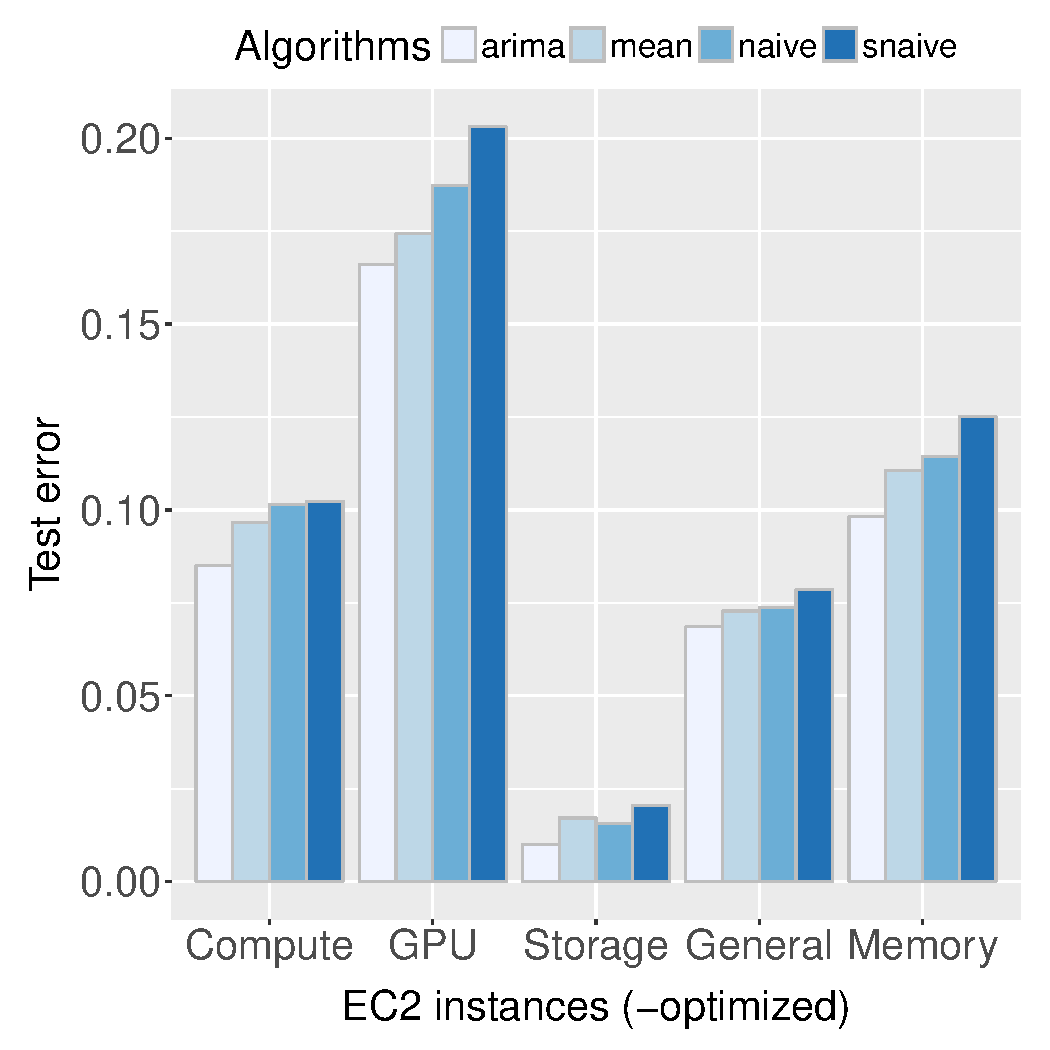
\includegraphics[width=0.7\textwidth]{figures/algorithm-compare-different-instance-type.pdf}\caption{Algorithms with different instance types\label{fig:algo-diff-inst}}
\end{figure}

\section{Conclusion}
Summarize

%\begin{acknowledgement}
%Thanks to ...
%\end{acknowledgement}
\bibliographystyle{spmpsci}
\bibliography{g2-price-modeling}
\end{document}
